
% Copyright 2004 by Till Tantau <tantau@users.sourceforge.net>.
%
% In principle, this file can be redistributed and/or modified under
% the terms of the GNU Public License, version 2.
%
% However, this file is supposed to be a template to be modified
% for your own needs. For this reason, if you use this file as a
% template and not specifically distribute it as part of a another
% package/program, I grant the extra permission to freely copy and
% modify this file as you see fit and even to delete this copyright
% notice. 

\documentclass{beamer}
\usepackage[utf8x]{inputenc}
\usepackage{graphicx}
\graphicspath{ {./image/} }

% There are many different themes available for Beamer. A comprehensive
% list with examples is given here:
% http://deic.uab.es/~iblanes/beamer_gallery/index_by_theme.html
% You can uncomment the themes below if you would like to use a different
% one:
%\usetheme{AnnArbor}
%\usetheme{Antibes}
%\usetheme{Bergen}
%\usetheme{Berkeley}
%\usetheme{Berlin}
%\usetheme{Boadilla}
%\usetheme{boxes}
%\usetheme{CambridgeUS}
%\usetheme{Copenhagen}
%\usetheme{Darmstadt}
%\usetheme{default}
%\usetheme{Frankfurt}
%\usetheme{Goettingen}
%\usetheme{Hannover}
\usetheme{Ilmenau}
%\usetheme{JuanLesPins}
%\usetheme{Luebeck}
%\usetheme{Madrid}
%\usetheme{Malmoe}
%\usetheme{Marburg}
%\usetheme{Montpellier}
%\usetheme{PaloAlto}
%\usetheme{Pittsburgh}
%\usetheme{Rochester}
%\usetheme{Singapore}
%\usetheme{Szeged}
%\usetheme{Warsaw}

\title{Projet PROG6}

% A subtitle is optional and this may be deleted
\subtitle{Pingouins}

\author{A.~Castel \and C.~Eymond Laritaz \and G.~Sorin \and L.~Soret \and T.~Vandendorpe \and P.~Reboul}
% - Give the names in the same order as the appear in the paper.
% - Use the \inst{?} command only if the authors have different
%   affiliation.

\institute[Université Grenoble-Alpes] % (optional, but mostly needed)
{
  UFR IM²AG\\
  Université Grenoble-Alpes
}
% - Use the \inst command only if there are several affiliations.
% - Keep it simple, no one is interested in your street address.

\date{Vendredi 1 Juin 2018}
% - Either use conference name or its abbreviation.
% - Not really informative to the audience, more for people (including
%   yourself) who are reading the slides online

% logo of my university
\titlegraphic{
 {\centering
 \vspace{-1.5cm}
 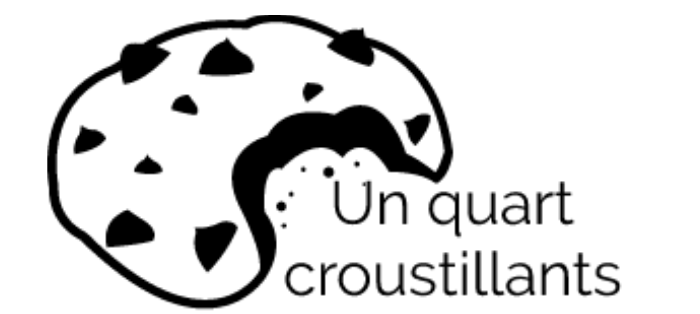
\includegraphics[height=1cm]{logoUnQuart}\hspace*{6.5cm}~%
 
\includegraphics[height=1cm]{logo_im2ag}
 }
}

\subject{Informatique}
% This is only inserted into the PDF information catalog. Can be left
% out. 

% If you have a file called "university-logo-filename.xxx", where xxx
% is a graphic format that can be processed by latex or pdflatex,
% resp., then you can add a logo as follows:

%\pgfdeclareimage[height=0.7cm]{team-logo}{logo_team.png}
%\logo{\pgfuseimage{team-logo}}

% Delete this, if you do not want the table of contents to pop up at
% the beginning of each subsection:
\AtBeginSubsection[]
{
  \begin{frame}<beamer>{}
    \tableofcontents[currentsection,currentsubsection]
  \end{frame}
}

% Let's get started
\begin{document}

\begin{frame}
  \titlepage
\end{frame}

\begin{frame}{Outline}
  \tableofcontents
  % You might wish to add the option [pausesections]
\end{frame}

% Section and subsections will appear in the presentation overview
% and table of contents.
\section{IHM}

\subsection{Menu}

\begin{frame}{Les menus}
  \begin{block}{Identification des besoins principaux}
	\begin{itemize}
	\item <1-> Creer une partie rapide (avec les règles de base)
	\item <2-> Naviguer entre les différents menus (boutons quitter, retour au menu précédent)
  	\end{itemize}
  \end{block}
\end{frame}

\begin{frame}{}
  \begin{block}{Identification des besoins secondaires}
	\begin{itemize}
	\item <1-> Pouvoir charger une partie précédemment sauvegardée
	\item <2-> Pouvoir jouer sur des terrains personnalisés
	\item <3-> Configurer et modifier les règles du jeu avant une partie
  	\end{itemize}
  \end{block}
\end{frame}

\begin{frame}{}
  \begin{block}<1->{Contraintes d'ergonomie}
	\begin{itemize}
	\item <1-> Lancer une partie en deux clics ou moins
	\item <2-> Pouvoir facilement configurer les règles du jeu si on recherche une expérience de jeu plus avancée
  	\end{itemize}
  \end{block}
  \begin{block}<3->{Configurations des règles}
	\begin{itemize}
	\item <3-> Supprimer et rajouter des joueurs
	\item <4-> Changer le type des joueurs (IA/Humain)
	\item <5-> Changer le nombre de pingouins de chaque joueur individuellement
	\item <6-> Changer la proportion de cases à un, deux ou trois poissons
	\item <7-> Changer les dimensions du plateau de jeu
  	\end{itemize}
  \end{block}
\end{frame}

\begin{frame}{Tests d'IHM}
  \begin{block}{Déroulé}
	\begin{itemize}
	\item <1-> Objectifs donnés aux testés
	\item <2-> Mesure de leur capacité/facilité à remplir les objectifs
	\end{itemize}
  \end{block}
\end{frame}

\begin{frame}{De la maquette à la version finale}
  \begin{block}<1->{Maquette de début de projet}
	\begin{itemize}
	\item <1-> Disposition et apparence des menus
	\item <2-> Présence des options qui peuvent vraisemblablement se trouver dans le jeu final
	\item <3-> Maquette intéractive (LibreOffice Impress)
  	\end{itemize}
  \end{block}
  \begin{block}<4->{Retours de tests d'IHM}
    \begin{itemize}
	\item <4-> Interface claire et lisible
	\item <5-> Placement des boutons intuitif
	\end{itemize}
  \end{block}
\end{frame}

\begin{frame}{De la maquette à la version finale}
  \begin{block}<1->{IHM de fin de projet}
	\begin{itemize}
	\item <1-> Implémentation de la maquette en tenant compte des retours
	\item <2-> Supression des fonctionnalités superflues
	\item <3-> Ajout de fonctionnalités importantes (chargement de terrains...)
  	\end{itemize}
  \end{block}
  \begin{block}<4->{Retours de tests d'IHM}
    \begin{itemize}
	\item <4-> Interface claire et lisible
	\item <5-> Logique des menus cohérente
	\end{itemize}
  \end{block}
\end{frame}

\subsection{Scene de jeu}

% You can reveal the parts of a slide one at a time
% with the \pause command:
\begin{frame}{Le plateau de jeu}
  \begin{block}{Identification des besoins}
    \begin{itemize}
    \item <1-> Information sur le plateau (pingouins, cases détruites, ...)
    \item <2-> Information sur l'état courant des joueurs (joueur courant, scores, ...)
    \item <3-> Que doit faire le joueur?
    \item <4-> Que peut faire le joueur?
    \end{itemize}
  \end{block}
\end{frame}

\begin{frame}{}
  \begin{block}{Autres options}
    \begin{itemize}
    \item <1-> défaire/refaire
    \item <2-> suggestion
    \item <3-> Autres options (sauvegarder, charger, quitter, ...)
    \end{itemize}
  \end{block}
\end{frame}

\begin{frame}{Evolution}
    \begin{center}
      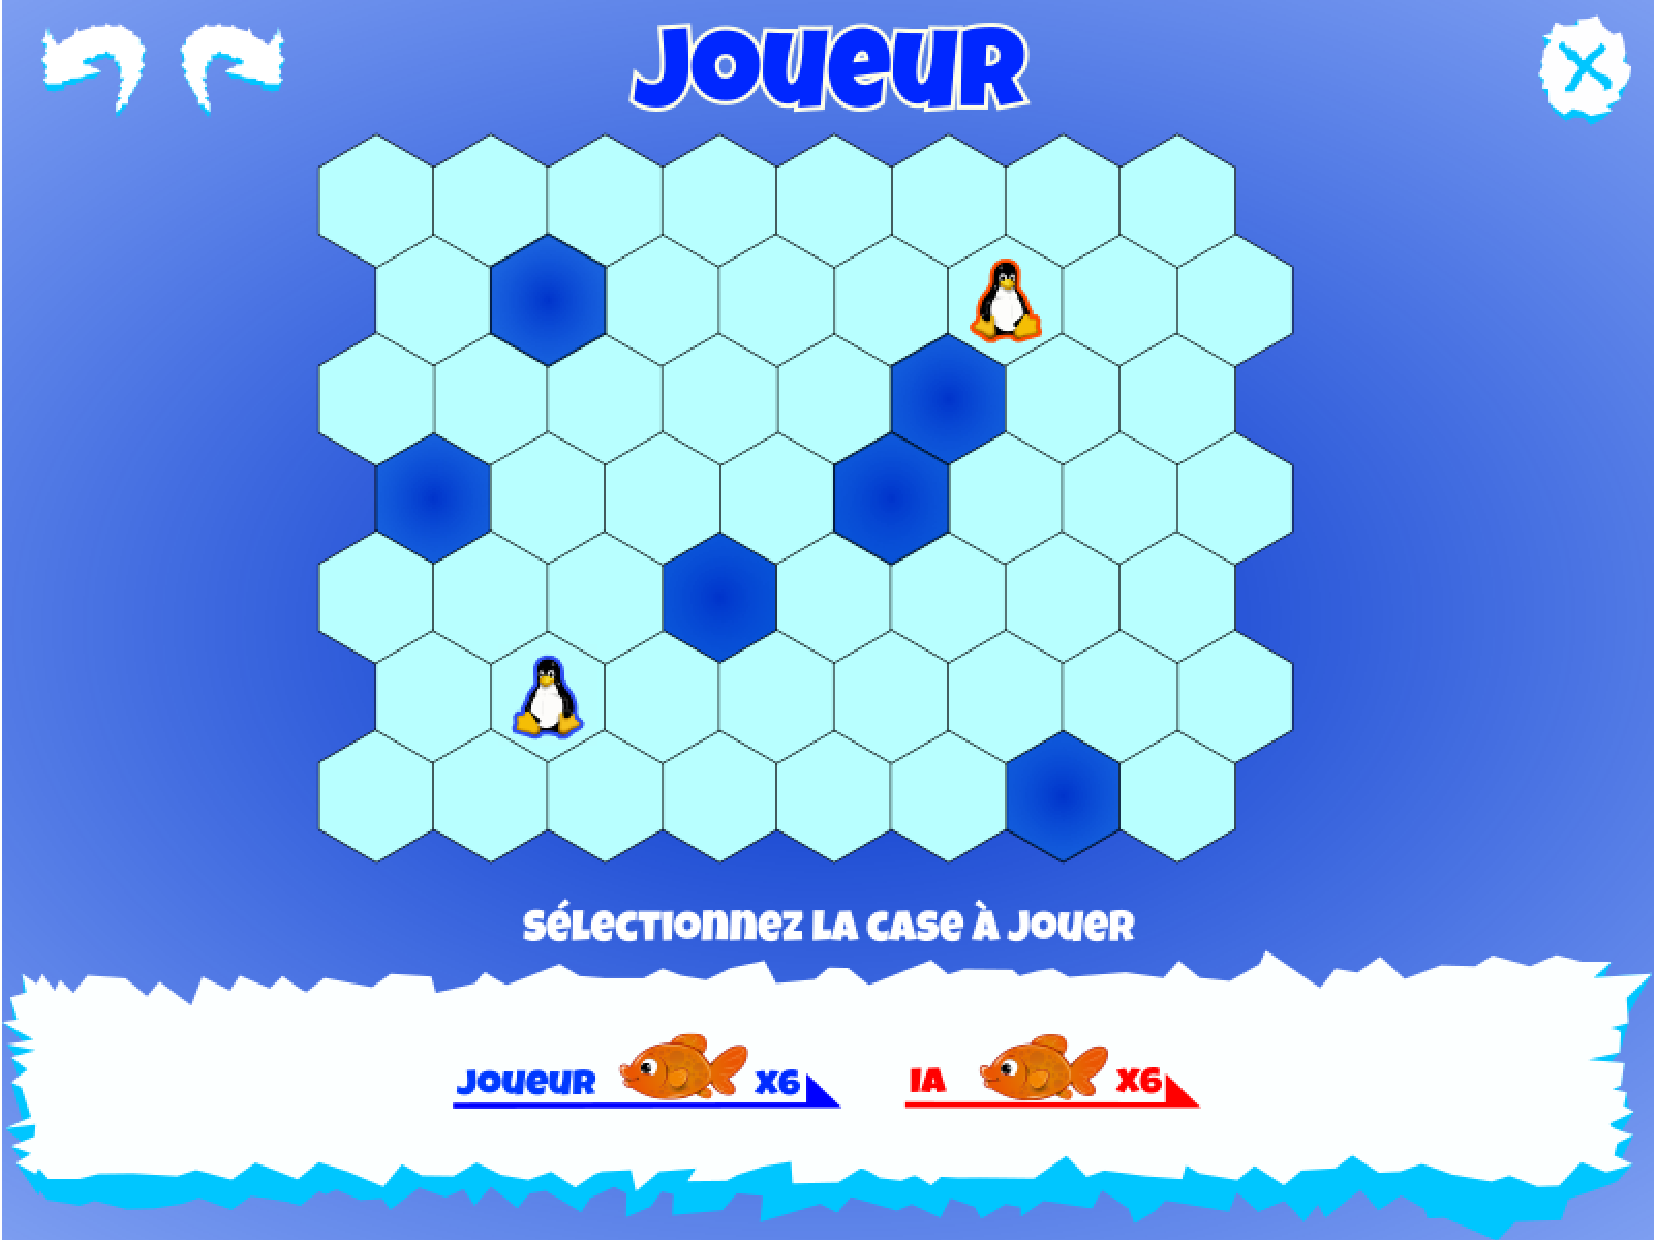
\includegraphics[scale=0.25]{ancienPlateau}
    \end{center}
\end{frame}

\begin{frame}{Résultat des tests IHM}
\begin{center}
 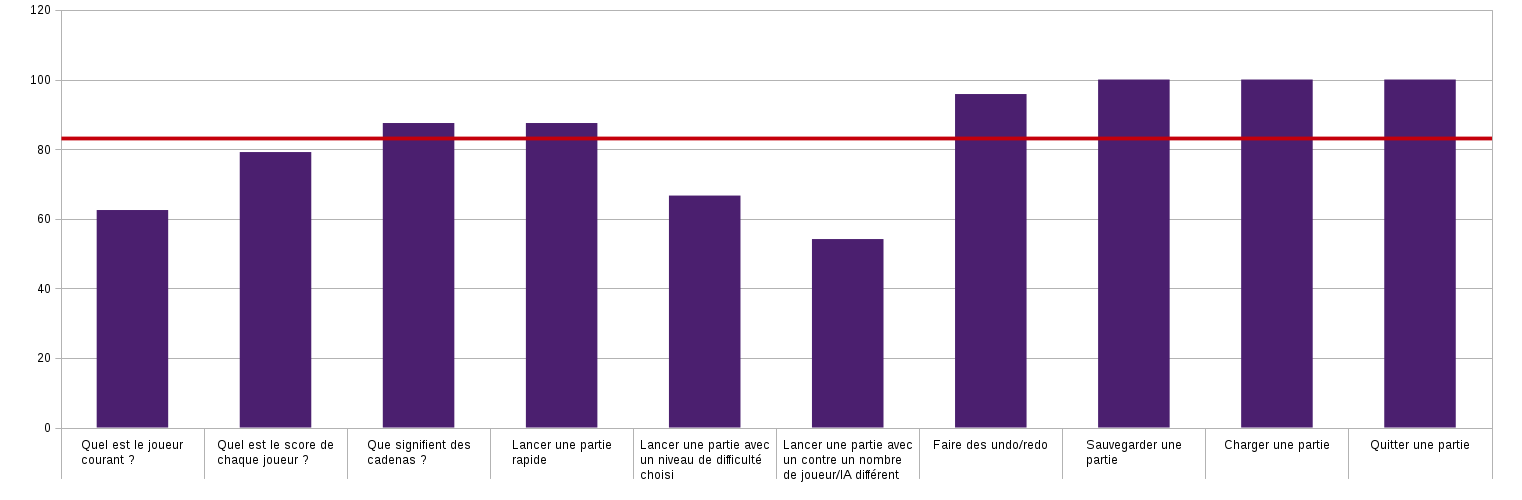
\includegraphics[scale=0.28]{graphIHM}
\end{center}
\end{frame}

\section{Aspects techniques}

%Tests JUnit

\subsection{Moteur}

\begin{frame}{Structure}
\begin{block}{}
\begin{itemize}
\item<1-> Automate à nombre d'états fini détérministe privé
\item<2-> Données privées sur l'état courant
\item<3-> Fonctions publiques qui modifient l'état selon les règles du jeu
\end{itemize}
\end{block}
\end{frame}

\begin{frame}{Automate à états fini détérministe}
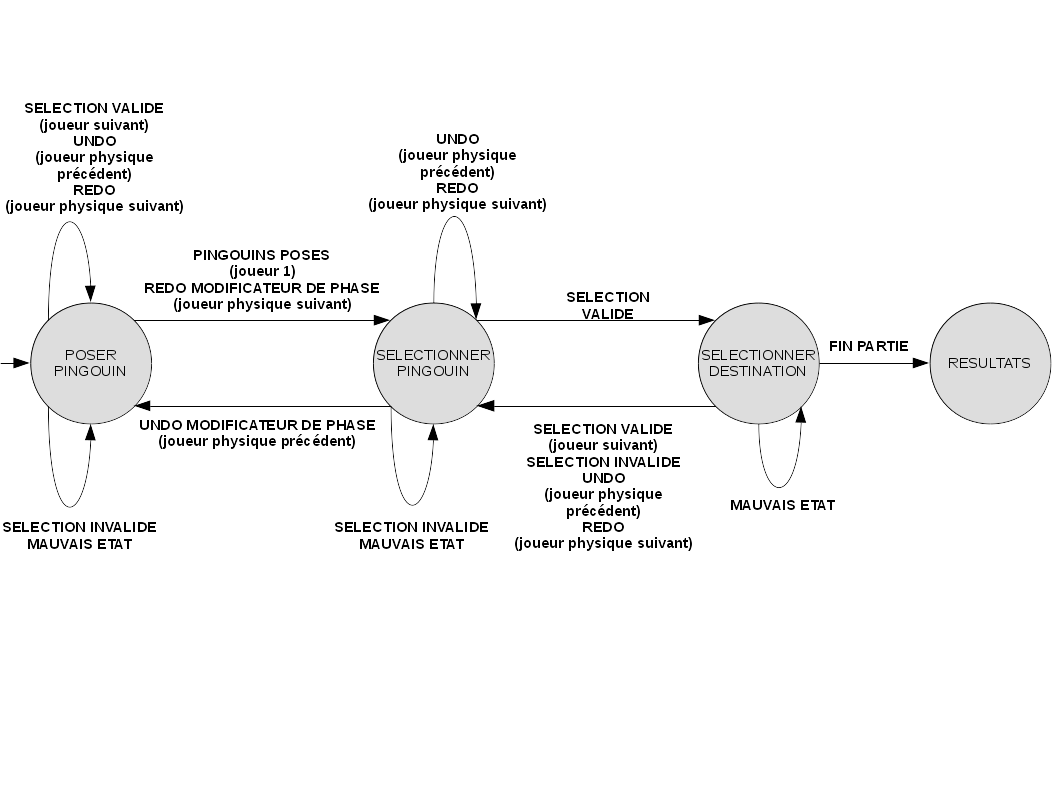
\includegraphics[scale=0.4]{AFD}
\end{frame}

\subsection{Génération de terrains}

\begin{frame}{}
\begin{block}{Choix possibles}
\begin{itemize}
\item<1-> Taille du terrain
\item<2-> Proportion de cases à 1,2 et 3 poissons
\item<3-> Chargement de terrains dans un format prédéfini
\item<4-> Génération paramétrée
\end{itemize}
\end{block}
\end{frame}

\subsection{Fonctionnalités}
\begin{frame}{}
\begin{block}<1->{Défaire/Refaire} %C'est l'undo-rados
Une classe Move pour stocker un coup \newline
Deux piles: 
\begin{itemize}
 \item historique des coups faits (défaire)
 \item historique des coups annulés (refaire)
\end{itemize}
\end{block}
\begin{block}<2->{Sauvegarde/Chargement}
\begin{itemize}
\item Complète
\item Non modifiable (données sérialisées)
\end{itemize}
\end{block}
\end{frame}

\begin{frame}{}
\begin{block}{Autres}
\begin{itemize}
\item<1-> Tests JUnit
\item<2-> Intelligence artificielle sur un thread à part
\end{itemize}
\end{block}
\end{frame}


\section{IA}

\subsection{Placement en début de partie}
\begin{frame}{}
\begin{block}{Placement en début de partie}
\begin{itemize}
 \item<1-> Le plus proche possible des bancs de poissons
 \item<2-> En evitant les bords autant que possible
 \item<3-> En essayant de bloquer l'ennemi autant que possible
 \item<4-> En essayant de ne pas coller tout ses poissons
\end{itemize}
\end{block}
\end{frame}

\begin{frame}{Placement en début de partie}
\begin{center}
 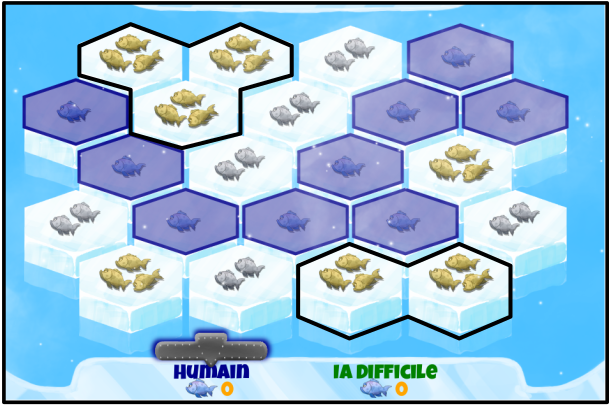
\includegraphics[scale=0.22]{IA1}\hspace*{0.5cm}~%
 \pause
 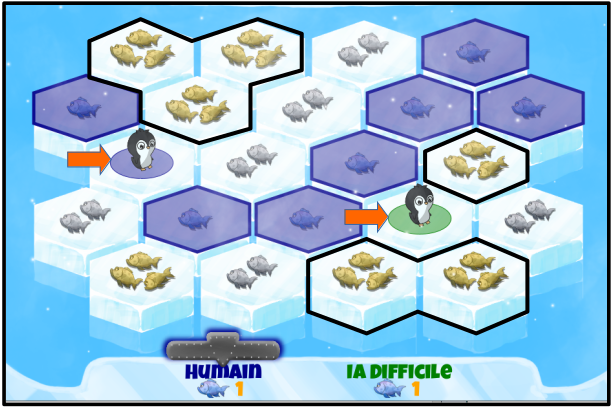
\includegraphics[scale=0.22]{IA2}
\end{center}
\end{frame}



\subsection{Évaluation des feuilles}

\begin{frame}{}
\begin{block}{Cas favorables}
\begin{itemize}
 \item<1-> Isoler un pingouin ennemi.
 \item<2-> Isoler tous les pingouins ennemis sur une îles suffisamment petite pour qu'il ne puisse pas gagner en fonction du score courant.
 \item<3-> Si la partie est finie et que notre score est le plus élevé.
\end{itemize}
\end{block}
\end{frame}

\begin{frame}{}
\begin{block}{Cas défavorables}
\begin{itemize}
 \item<1-> Avoir un pingouin isolé.
 \item<2-> Avoir tous nos pingouins isolés sur une île trop petit pour pouvoir gagner.
 \item<3-> Une grande île sans pingouins dessus.
 \item<4-> Si un ou plusieurs pingouins ennemis sont isolés sur une île suffisamment grande pour qu'ils s'assurent la victoire.
\end{itemize}
\end{block}

\begin{block}{}
\begin{itemize}
\item<5-> Calculs ajustés en fonction des scores.
\end{itemize}
\end{block}

\end{frame}

\subsection{Fin de partie}

\begin{frame}{}
\begin{block}{Fin de partie}
\begin{itemize}
  \item<1->{On fait un parcours Hamiltonien sur chaque île}
  \item<2->{Si c'est impossible, on essaie au moins de ne pas le briser}
\end{itemize}
\end{block}
\end{frame}

\subsection{IA facile et moyenne}
\begin{frame}{}
\begin{block}{IA facile}
\begin{itemize}
  \item<1->{Basée sur le placement en début de partie de l'IA difficile}
  \item<2->{Stratégie différente : On récupère le plus de poissons le plus vite possible}
\end{itemize}
\end{block}
\end{frame}
\begin{frame}{}
\begin{block}{IA Moyenne}
\begin{itemize}
  \item<1->{Principe et stratégie basés sur l'IA difficile}
  \item<2->{Calcul d'une partie plus petite de l'arbre}
\end{itemize}
\end{block}
\end{frame}

\subsection{Améliorations}
\begin{frame}{}
\begin{block}{Améliorations possibles pour l'IA difficile}
\begin{itemize}
 \item<1-> Multi-Threader le calcul de l’arbre
 \item<2-> Faire en sorte que l’IA difficile puisse changer de stratégie selon la situation
 \item<3-> Optimiser le calcul du parcours Hamiltonien
\end{itemize}
\end{block}
\end{frame}

\begin{frame}{}
\begin{block}{Améliorations testées et abandonnées}
\begin{itemize}
 \item<1-> Utiliser MinMax pour calculer le parcours Hamiltonien. 
 \item<2-> Calculer la profondeur a calculer de façon dynamique, pour chaque branches.
\end{itemize}
\end{block}
\end{frame}

\subsection{Tests}
\begin{frame}{}
\begin{center}

{
 \hspace*{1cm}~\tiny
 \textbf{\textit{Facile(Bleu) vs Difficile(Rouge) sur différents plateaux.}}
 \newline
 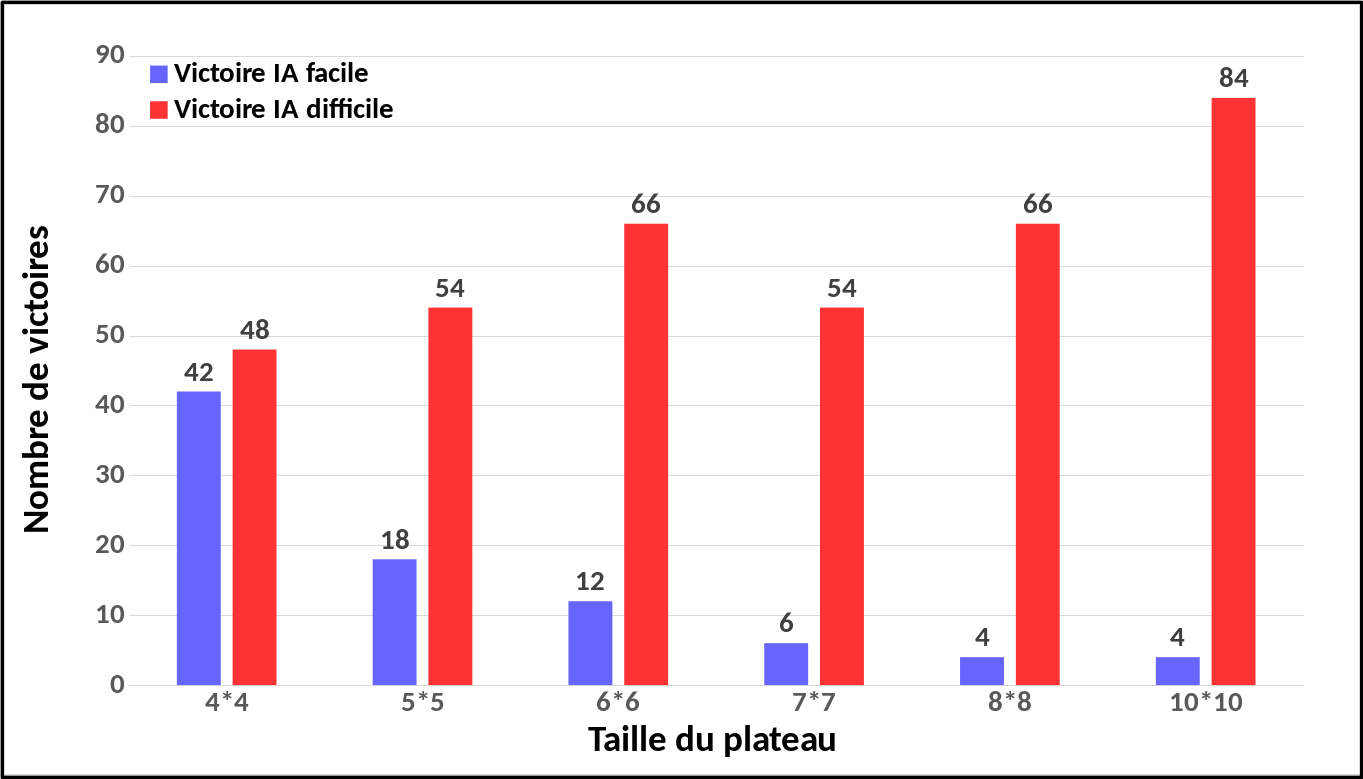
\includegraphics[scale=0.25]{IA10}
}

\end{center}
\end{frame}
\begin{frame}
\begin{center}


{ 
  \hspace*{1cm}~\tiny
 \textbf{\textit{Facile(Bleu) vs Moyenne(Rouge) sur différents plateaux.}}
 \newline
 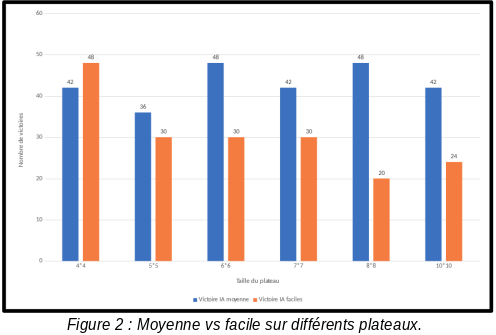
\includegraphics[scale=0.25]{IA11}
 }
 
\end{center}
\end{frame}


\begin{frame}{}
\begin{center}
{
 \hspace*{2cm}~\tiny
 \textbf{\textit{Humain(gris) vs Difficile(Rouge)}}
 \newline
 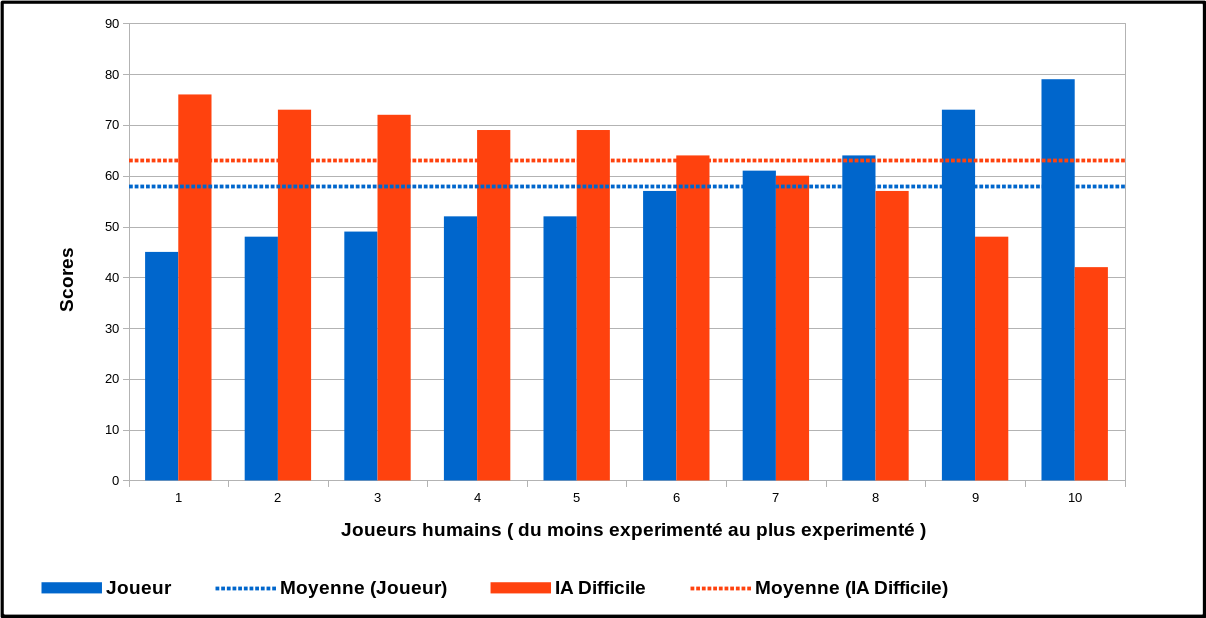
\includegraphics[scale=0.40]{IA12}
}
\end{center}
\end{frame}

\begin{frame}
 \begin{center}
  \Huge Merci de votre attention
 \end{center}
 \begin{center}
  
\includegraphics[scale=0.55]{pingouin}
 \end{center}
\end{frame}


\end{document}


